\chapter{Hackathons}\todo[size=\small]{Suggest combining the two last chapters into something like "Experience with Challenge-based learning events: from hackathons to student projects." Somehow, you need to link this more closely with the issue of documentation, and to connect to data and results that you have gathered. Same for the summer student part.}
% We're going to need an extra theorem-like environment for this
% chapter
\theoremstyle{plain}
\theoremsymbol{}
\newtheorem{Rule}[theorem]{Rule}

\begin{comment}
%%  A structure to follow in each section

% Abstract
\section{Abstract}

% Introduction
\section{Introduction}

%% Central Report Section
% Methodology
\section{Methodology (what you did/used)}

% RESULTS
\section{RESULTS (what you found/saw)}

% DISCUSSION/CONCLUSION
\section{DISCUSSION/CONCLUSION}

\renewcommand{\labelenumii}{\Roman{enumii}}
\begin{enumerate}

	\item  

\end{enumerate}
\end{comment}

%% Start Here 




\section{Introduction}
Open innovation continue to expand the space of innovation and shape a new model for knowledge exchange between innovative industries, research and development laboratory, non-profit organizations and open communities. Hackathons became a platform for open innovation around the world and a scene for creative firms and institutions to help them achieve and sustain innovation. A Hackathon is a periodic event where computer programmers and others in the field of software development such as graphic designers, interface designers, UX experts, project managers and others collaborate intensively over a short period of time on software projects. It is also known as a hack day, hack fest, code fest \cite{wiki:hackathon}. These hackathon are giving the chance for everyone to learn, create  and innovate. From participating in large numbers of hackathon in a large range of different spaces (open data, science hack, food hack, programming, and more). We first consider the origins of hackathons and its different formats, and that lead us to classify the different hackathon type that occur. We also look at the results of an analysis conducted of a 18 hackathon events we observed and participated. We then discuss the potential of open innovation events, including common general principles that we have observed. We conclude by contemplating the future and value of open innovation, especially in offering people the opportunity to meet and collaborate to build new liaison that extend beyond the short term focus of the event. Also the potential for open innovation for networking in new spaces, along with the emerging Festival of Hack. But there is a lack of documentation in these hackathons and open innovation events, many ideas are generated out of these events but we cannot find any trace of it or a continuation for the potential project that came out with.

Recently, researchers are paying attention to the use of the software development and code-hosting web service GitHub for other collaborative purposes. These alternative uses of GitHub as a platform for sharing non-code artifacts represent an important modification in the practice of open collaboration\cite{longo2015use}. But due to the limitations of GitHub as a platform for technical participant, We investigate in a platform called \textit{SDGinProgress} that is open for everyone and people with non technical skills to collaborate and share their project with others, identify its strengths and weaknesses when used in this mode, and propose conditions for successful collaborations on co-created project. Then we will see how created documentation could help in the future of the process in a long term perspective.

\section{Hackathon}

The term  \textquotedblleft hackathon\textquotedblright\ appeared first back at the end of 90s when a group of developers flock together from around the world, and they created the first IPv6 and IPSEC stack NNcompletely integrated into an operating system \cite{openbsd} within a week, and OpenBSD software developer’s use of the term referred to a cryptographic development event held in Calgary on 4th June 1999 where small number of developers came together to avoid the legal problems arising from export regulations of cryptographic software from the United States of America (USA). A hackathon is an event in which computer programmers, system engi neers and others (graphic designers, interface designers and others) collaborate intensively over short period of time on software projects.

Hackathons became more widespread in the mid to late 2000s, increasingly attract companies, organisations and venture capitalists as a way to drive innovation, develop new software technologies and to discover new areas of funding. The hackathon movement have been growing while developing its organization from their impromptu pizza parties origins to professionally organised corporate sponsored bespoke events \cite{briscoe2014hackathon}. This has influenced the culture of innovation among companies and lead them to use  hackathons to innovate because of its effectiveness \cite{AnnaCordes2014}. The growth occurrence of hackathons around the globe and their effectiveness has lead to consider hackathons as an event that have significant impact of the culture of innovation and we will describe more the development of the culture of innovation. Also we are going to classify hackathon according to the them and format that take and we will and we will finish by sharing our finding about the incentive of writing and why is the lack of documentation.

\section{Format}
Generally, hackathons are one day or two days events. they start with pitching ideas, team are formed based on members individual interests and skills. At the end of the hackathon, each group presents their results in different format (demo of a prototype or presentation of the progress that has been done). The challenges or ideas can be announced before the event by the organizers or collected from the participants before the hackathon. Alternatively, a general topic could be suggested by the organizers and challenges/ideas could be generated at the event. Some hackathons include team building or ice breaking session e.g. in between pitching ideas and team matching to give the opportunity for participants to learn more about the ideas from others and to facilitate the team matching.

\section{Potential of Hackathons}
Hackathon became a genuine link between research and development, start-ups and the innovation world where people put together the laboratory setting and the field. Hackathons are a special place to think differently because it acts dynamically, it is characterized by constant change, activity, and progress \cite{Thesishackinnovation2015}. The organizational forces that impel a team or a project to be shaped beforehand does not exist. People from different backgrounds project their interdisciplinary knowledge on a selected topic they choose to tackle with different range of magnitude that make up the innovation process. During one two or two days hack, participants find themselves in a decision environment that is complex, time pressure, spontaneously evolving and changing information and high information ambiguity. This environment drives them to iterate quickly over their idea, prototype it and see the result. This iteration process propels their idea/prototype to a new level that make up their innovation unique. Participants in a hackathon contribute to the project and to the team effort, as max as they can, since the outcome gives them visibility and creates new opportunities and gives them a professional reputation.

These characteristics allow companies, corporations, academia to follow this model to help them innovate and sustain their creativity within an environment of high competition where they are always seeking new ideas, new products to offer to their customers. Also, hackathons have great potential to offer people the opportunity to explore new ideas, to learn about new areas and to make products in a short period without dealing with obligation and pressure to deliver. If this model of innovation is efficient and productive for industry, more effort need to be put down to find how we can encourage more areas of work to adapt this model to innovate and create in their field.

\section{Classification}
Hackathons are increasingly adapted by more environment, they don't have a specific focus or participants and organizers leave the participants to choose what to focus on. Hackathons focus on different aspects or topics. With the adaptation of the model of hackathons by the firms, institutions, NGO and more that work in different areas, hackathons started to be more oriented toward a specific topic. Based on our experience in the 17 hackathons and the 3 experiments of open geneva -open geneva is a festival of innovation where more hackathons occur on the same city in Geneva- we classified the hackathons as following Designathon, Humathon, Digithon, Codithon, Concepthon and Learnathon. Designthons are hacakthons that focus on design, Humathons for humanitarian hackathons, Codithon, Learnathon that focus on learning new skill
 and more

\begin{center}
	\begin{tabular}{ |c|c|c| } 
		\hline
		Designathon & 2  \\ 
		Humathon & 6 \\ 
		Digithon & 11 \\ 
		Codithon & 18 \\
		Concepthon & 5 \\ 
		Learnathon & 3\\ 
		\hline
	\end{tabular}
\end{center}

 \begin{comment}
 
\section{Rubbish}
\Rule{What is it ?}
How it works in hackathons with people from different backgrounds, how ideas get generated and how people document their hackathons ?
key words : 
The term hackathon appeared in 1991, 
knowledge exchange, digital creative industries, creative economy, culture hacks, technology hack, food hack, potential of X- hack , innovative, prototypes, digital, interdisciplinary people, different backgrounds, application of hackathon to humanitarian goals, applying professional practice to their research, potential of humanitarian hack in Geneva, knowledge exchange between technology, science and humanities and the digital creative industries.

The hackathon model changed over the past decade as people find out it could foster innovation, bring new insight to the tech industry etc..
innovation with digital technologies come to the fore


over the 

\paragraph{new way to the problem of innovation}
Companies and other institutions take a new way to the problem of innovation within their research and development 
Expanding the space for innovation continue 
The exploration of open innovation for innovation exchange and expands the space for innovation



\end{comment}
\section{Open Geneva}
Open Geneva has been established to promote open innovation with a spirit of knowledge sharing for the common good. In particular, Open Geneva aims to foster open innovation for the arts, science, technology, and for society in the Greater Geneva Area. Open Geneva was established in 2015 by the Geneva Creativity Center in order to promote innovation for the improvement of life quality in Geneva. During the 1st edition, several teams of students worked during 2 weekends on scientific projects, as well as social and technical innovations, related to energy, health, mobility. The 2016 edition was focused on medical technologies and brought a larger scope of participants during a curated hackathon organized by The Port in collaboration with the Geneva University Hospitals\cite{web:opengeneva}.
Open Geneva started with one hackathon at the computer science department at University of Geneva with a crowd of more then 40 participants. The initiative get the attraction of more companies and institution in Geneva and in 2017, there were more then 20 hackathon with more then 400 participants. We were afraid that if we organize more hackathons, it will not be easy to find participants but it turns out that more you organize hackathons, the more people you have. And, this year there were more then 30 hackathon organized around the city with more then 800 participants and here we see an exponential growth of hackathon and participants

I\begin{figure}[H]
	\centering
	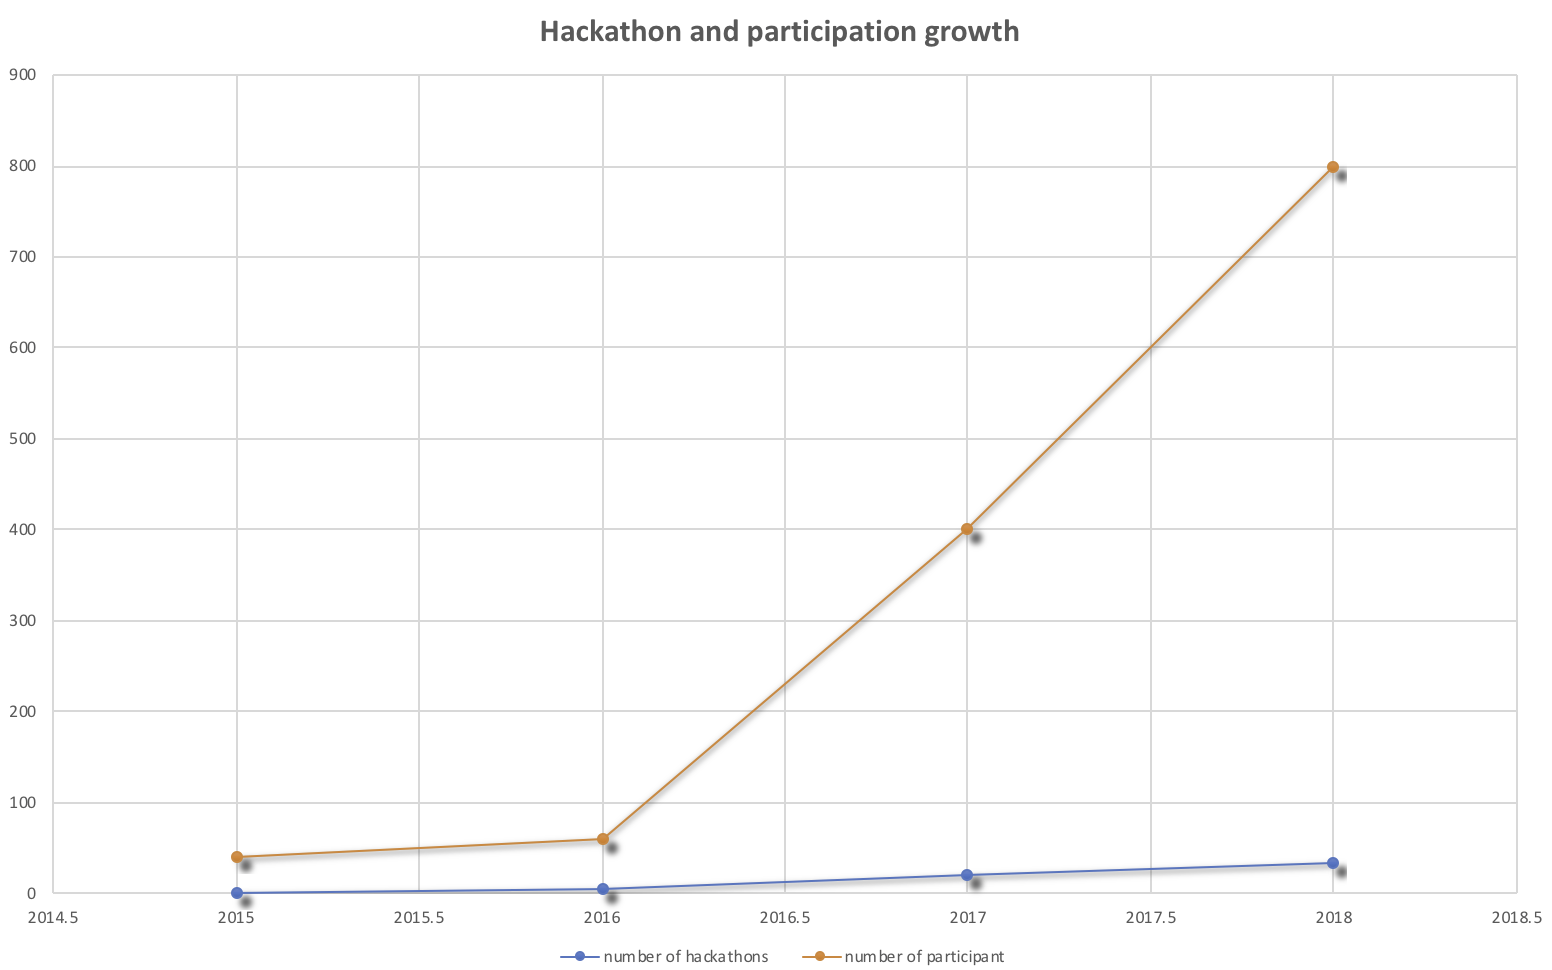
\includegraphics[scale=.4]{./images/img-hackstat.png}
	\label{img-hackstat}
	\caption{}
\end{figure}
\todo[size=\small]{The figure needs a caption, and text on axes is not readable. Is this your data}


\section{DISCUSSION/CONCLUSION}

\renewcommand{\labelenumii}{\Roman{enumii}}
\begin{enumerate}

	\item Summarize experience of hackathons / personal point of view
	\item Write about this experience and what you came out with
	\item Democratize innnovation

\end{enumerate}

%%% Local Variables:
%%% mode: latex
%%% TeX-master: "thesis"
%%% End: